\chapter{Equipment} \label{ch:equipment}
%head
For the robot to be able to navigate amongst humans it must be able to sense its surroundings. As described in section \ref{ch:HRI} about HRI, the robot must be able to distinct humans from static objects and must be able to keep a certain distance from humans. Therefore, the robot must be equipped with sensors that enables the detection of humans, objects and localises the position of these. This means the sensors must be able to calculate the distance from the sensor to the detected object. Common approaches to object detection are 2D range-based sensors and RGB-D cameras, as described by R. Triebel et al. \cite{SPENCER_paper}. As test platform a robotic solution named Turtlebot 2 was chosen.\\


\section{SICK TIM571}
%lidar in general
Light Detection and Ranging (LIDAR) is an active sensor, which means that this sensor does not need any light-source since it is emitting a laser pointer that is continuously firing on a surface and measuring the time for the laser to bounce back to calculate the distance, which is the principal of time of flight (TOF). 
 
\begin{figure}[H]
    \centering
    \begin{minipage}[b]{0.64\linewidth}
        In most LIDARs the laser is controlled by a mirror that determines where the pulses of light is emitted. There are particular LIDARs that use different light emitting pulses, one of them being  micropulses. The lasers used in LIDARs are categorised by wavelengths, where 600-1000nm can be used for safety purposes. 1550nm is an alternative that does not hurt the eye. This wavelength has lower accuracy and higher range \cite{Lidarwork}.
        The LIDAR SICK TIM571 shown in figure \ref{fig:sicktim571}, has a wavelength of 850nm which is infrared light. The horizontal field of view of the LIDAR is 270\degree, with a working range of 0.05m to 25m \cite{2dlidar}.
    \end{minipage}
    \hspace{0.2cm}
    \begin{minipage}[b]{0.33\linewidth}
        \centering
    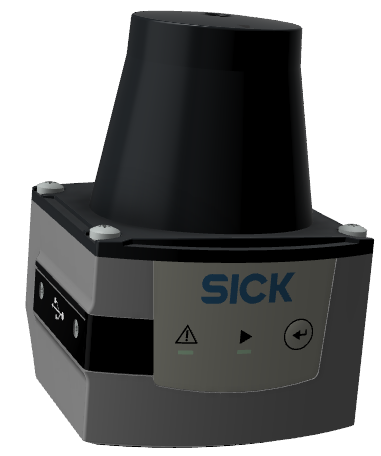
\includegraphics[width=\textwidth]{figures/TIM571-LIDAR.png}
    \caption{A LIDAR from SICK type TIM571. This LIDAR can messeaure a distance to a point in a 270\degree FOV at a distance of 0.05m to 25 m. \cite{2dlidar} }
    \label{fig:sicktim571}
    \end{minipage}
\end{figure}
% \begin{figure}[H]
%     \centering
%     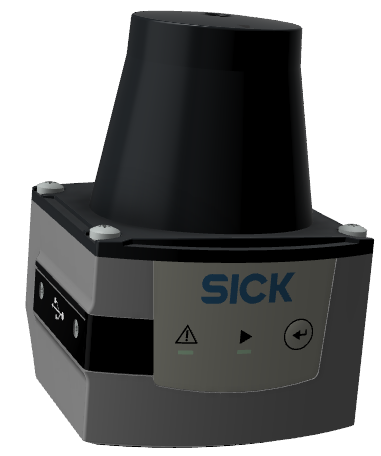
\includegraphics[width=.75\textwidth]{figures/TIM571-LIDAR.png}
%     \caption{An image of the SICK TIM571}
%     \label{fig:sicktim571}
% \end{figure}
To measure the distances from the LIDAR, the High Definition Distance Measurement (HDDM) method is used. This principle is a TOF principle that determines the travel time for each laser pulse the LIDAR emits. However the HDDM provides a measurement process that can evaluate each laser pulse statistically and determine the distance.
The statistically HDDM method is being used to measure multi-echo capability to implement in the sensors. This can sort out the most relevant echo to select, which gives the LIDAR a good certainty of the environment even in ambient conditions \cite{HDDM}.\\
% Why do we use it. (can be altered)
The SICK TIM571, in this project, is used for detection of round and elongated objects e.g. legs, as well as for detecting the environment of the robot. When the mobile robot helper moves around and help people it is able to recognise these objects to avoid collision and also when the robot is mounted with a camera it can be fused with the LIDAR to determine recognition of a person, e.g. the detection of legs and facial detection combined or separately should trigger the robot to believe it is a person it is detecting.\\

The determination of a person standing with the front or the back to the robot is where the other sensors can be utilised, because the LIDAR will have difficulties by distinguishing the front of the legs or the back of them. The determination of different people in the field of view can be determined by pairing the legs by the distance between the legs, which can be read about in \ref{sec:LegDetect}.
% how do we use it

\section{RealSense D435}

Like the LIDAR, the RealSense camera from Intel is also an active sensor. The RealSense camera is a Red, Green, Blue, Depth(RGB-D) camera and can be seen on figure \ref{fig:realsense}. Being a RGB-D camera means that the RealSense camera have a coloured image camera and it can calculate depth. The depth is not acquired from the coloured camera but the two Infra-Red(IR) cameras, that is used in a stereo vision manner, and a laser that is projecting an IR pattern.\cite{RealSense}\\

\begin{figure}[H]
    \centering
    \begin{minipage}[b]{0.58\linewidth}
    The RealSense also enables tracking, based on the input from the IR cameras, which can be useful for gathering data on the movement of people.\cite{RealSense}\\
    Some of the reason why this RealSense was chosen over other well know RGB-D cameras as the Microsoft Kinect, which was used in the Spencer robot, or the ASUS Xtion, is the depth viewing capabilities and the field of view (FOV) of the RealSense. 
    \end{minipage}
    \hspace{0.2cm}
    \begin{minipage}[b]{0.39\linewidth}
    \centering
    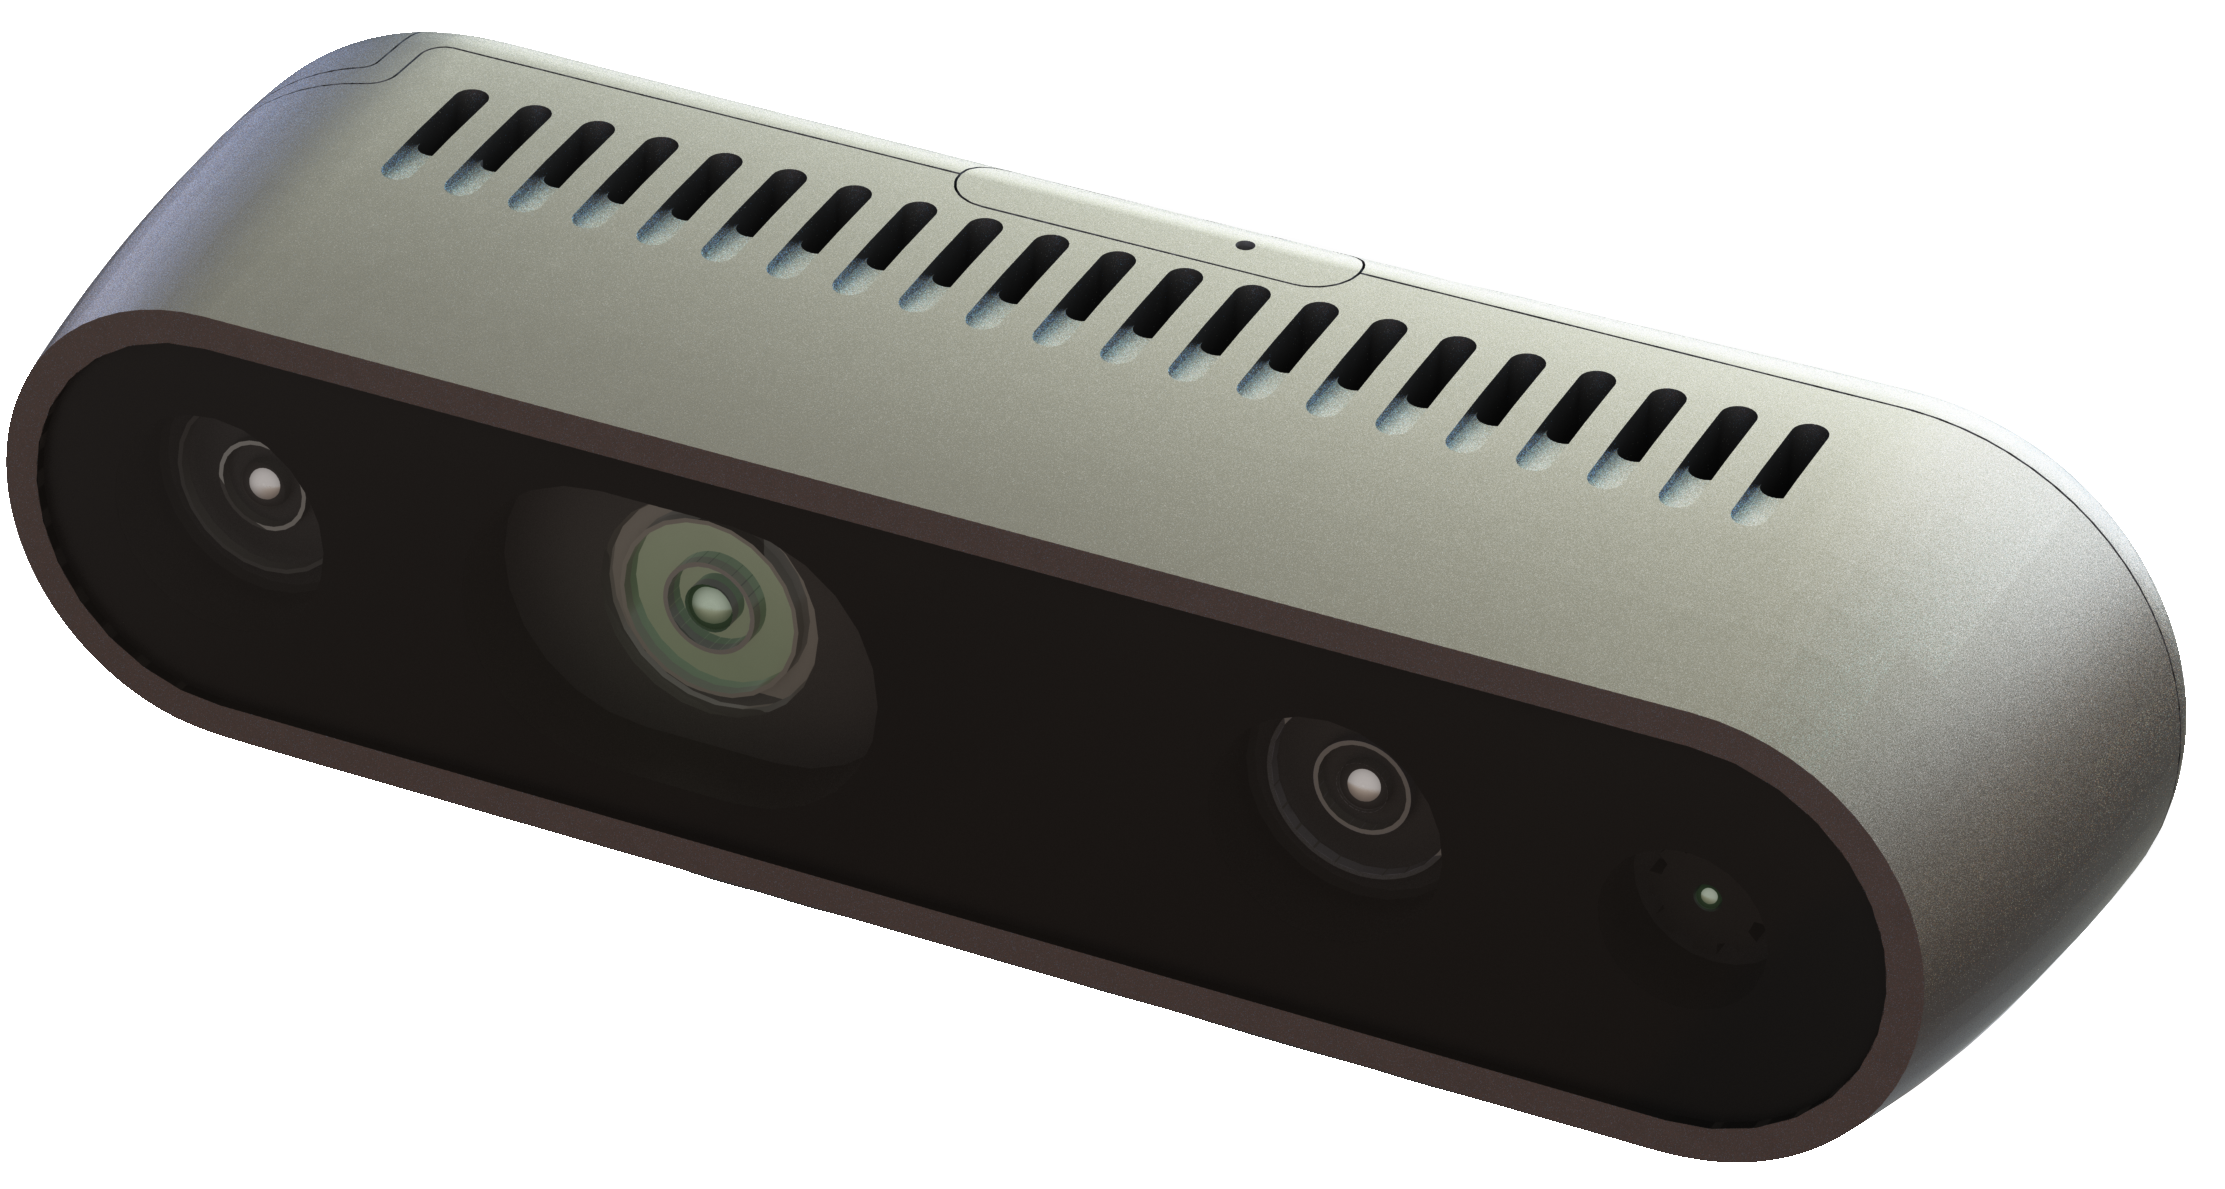
\includegraphics[width=\textwidth]{figures/IntelRealsense.png}
    \caption{The RealSense D435 camera from Intel. A camera that can capture a coloured image as well capturing the depth of the scene.  }
    \label{fig:realsense}
    \end{minipage}
\end{figure}

It has a depth viewing distance from 0.1 m up to 10 m depending on the environment's illumination\cite{RealSense}, wheres as the Kinect has from 1.2 meters and the Xtion camera has from 0.3 and both up to 3.5 meters\cite{Xtion}\cite{Kinect} depending on the illumination. The FOV horizontal for the RealSense is 87\degree and 58\degree vertical where as Xtion has 58\degree horizontal, 45\degree vertical\cite{Xtion} and Kinect 57\degree horizontal, 43\degree vertical\cite{Kinect}. Moreover the RealSense camera can capture more frames per second than the other two aforementioned cameras, which will provide more depth information, and it can be used in outdoor and indoor illuminated scenes.\cite{RealSense} \\

The RealSense is used for face detection to compliment the leg detection from the LIDAR. This helps ensure the detection of people when moving around in a hypermarket. With the sensors chosen for this project the mobile robot platform used will be described.
